\documentclass{beamer}

\mode<presentation>
{
  \usetheme{Warsaw}
  \setbeamercovered{transparent}
}

\usepackage[english]{babel}
\usepackage[latin1]{inputenc}
\usepackage{times}
\usepackage[T1]{fontenc} 
% Or whatever. Note that the encoding and the font should match. If T1
% does not look nice, try deleting the line with the fontenc.
\usepackage{amsmath}

\newcommand{\linespace}{\vskip 0.25cm}

\definecolor{MyForestGreen}{rgb}{0,0.7,0} 
\newcommand{\tableemph}[1]{{#1}}
\newcommand{\tablewin}[1]{\tableemph{#1}}
\newcommand{\tablemid}[1]{\tableemph{#1}}
\newcommand{\tablelose}[1]{\tableemph{#1}}

\definecolor{MyLightGray}{rgb}{0.6,0.6,0.6}
\newcommand{\tabletie}[1]{\color{MyLightGray} {#1}}

% The text in square brackets is the short version of your title and will be used in the
% header/footer depending on your theme.
\title[Usability of error messages for introductory students]{Usability of error messages for \\ introductory students}

% Sub-titles are optional - uncomment and edit the next line if you want one.
% \subtitle{Why does sub-tree crossover work?} 

% The text in square brackets is the short version of your name(s) and will be used in the
% header/footer depending on your theme.
\author[Schliep]{Paul Andrew Schliep}

% The text in square brackets is the short version of your institution and will be used in the
% header/footer depending on your theme.
\institute[U of Minn, Morris]
{
  Division of Science and Mathematics \\
  University of Minnesota, Morris \\
  Morris, Minnesota, USA
}

% The text in square brackets is the short version of the date if you need that.
\date[April '15] % (optional)
{25 April 2015 \\ University of Minnesota, Morris}

% Delete this, if you do not want the table of contents to pop up at
% the beginning of each subsection:
\AtBeginSection[]
{
  \begin{frame}<beamer>
    \frametitle{Outline}
    \tableofcontents[currentsection, hideothersubsections]
  \end{frame}
}

\begin{document}

\begin{frame}
  \titlepage
\end{frame}

% For a 20-25 minute senior seminar talk you probably want something like:
% - Two or three major sections (other than the summary).
% - At *most* three subsections per section.
% - Talk about 30s to 2min per frame. So there should probably be between
%   15 and 30 frames, all told.

\section*{Introduction}

\subsection*{Overview of error messages}

\begin{frame}[fragile]
  \frametitle{Introduction to error messages}
  \begin{itemize}
  	\item In programming, an error is when the computer cannot understand an expression in the code
  	\begin{itemize}
  		\item these errors will return an error message
  	\end{itemize}
  	\item Here's an example of an error message:
  	  \begin{verbatim}
  print("Hello World";
  ->java.3: error: unclosed string literal
  	\end{verbatim}
  \end{itemize}
\end{frame}

\begin{frame}
  \frametitle{Importance of error messages}
  \begin{itemize}
  	\item Error messages are important tool for beginner programmers
  	\begin{itemize}
  		\item one of the primary interactions between the system and the user
  	\end{itemize}
  	\item Unhelpful error messages impose learning difficulties, especially for new programmers
  	\item Error messages with poor usability can lead the user down the wrong path
  \end{itemize}
\end{frame}

\begin{frame}[fragile]
  \frametitle{Goals of an error message}
  \begin{itemize}
  	\item An error message should:
  	\begin{itemize}
  		\item not add confusion
  		\item be easy to understand
  		\item help a student locate the issue
  	\end{itemize}
  	\item Example:
  	\begin{verbatim}
  	Developing...
  	\end{verbatim}
  \end{itemize}
\end{frame}

\begin{frame}
 \frametitle{Analyzing error messages}
 \begin{itemize}
 	\item Human-computer interaction: study on interfaces between user and programs
 	\item Much of the research presented from an HCI perspective
 	\item We will discuss error messages in terms of usability
 \end{itemize}
\end{frame}

\subsection*{Outline}

\begin{frame}
  \frametitle{Outline}
  \tableofcontents[hideallsubsections]
\end{frame}

\section[Background]{Background}

\subsection{Compiler and runtime errors}

\begin{frame}[fragile]
	\frametitle{Compiler errors}
		\begin{itemize}
			\item When a compiler fails to compile a program, a user will receive a compiler error message
			\item For newer programmers, these typically occur from syntax errors
			\item Example (in Java):
			\begin{verbatim}
		int seven = (2 + 5;
		error: ')' expected
			\end{verbatim}
		\end{itemize}
\end{frame}

\begin{frame}[fragile]
	\frametitle{Runtime errors}
		\begin{itemize}
			\item A runtime error occurs after a program has compiled
			\item Usually indication of logical errors in the code
			\item Cannot be predicted, dependent on the values
			\item Example:
			\begin{verbatim}
			String string = "Hello World";
System.out.print(string.substring(6,12));

java.lang.StringIndexOutOfBoundsException:
String index out of range: 12
			\end{verbatim}
		\end{itemize}
\end{frame}

\subsection{Dynamic and statically typed}

\begin{frame}[fragile]
  \frametitle{Statically typed}
	\begin{itemize}
		\item All variables and/or objects assigned types
		\item Type checking done at compile time
		\begin{itemize}
			\item this means different error messages
		\end{itemize}
		\item Languages like Java or C++ are statically typed
		\item The following example would give an error at compile time in statically typed:
		\begin{verbatim}
		personName = "Frank"
		personName = 7
		\end{verbatim}
	\end{itemize}
\end{frame}

\begin{frame}[fragile]
  \frametitle{Dynamically typed}
	\begin{itemize}
		\item Values are not assigned to types
		\item Type checking done at runtime
		\item Languages in Lisp family
		\item The following example would give an error at runtime in dynamically typed:
		\begin{verbatim}
		personName = "Frank"
		personName = 7
		\end{verbatim}
	\end{itemize}
\end{frame}

\section[Analyses]{Analyses of error messages}

\subsection[DrRacket Analysis]{Analysis of DrRacket IDE}


\begin{frame}
  \frametitle{Overview of study}
  \begin{itemize}
  	\item Marceau et al. noticed students struggling with error messages in course
  	\item Conducted study on DrRacket error messages in Spring of 2009
  	\item Hoping to use the data to improve students' interactions with DrRacket error messages
  \end{itemize}
\end{frame}

\begin{frame}
	\frametitle{Integrated development environments}
		\begin{itemize}
			\item An integrated development environment (IDE) is a program for writing and running code
			\item Some IDEs come packaged with debugging tools and custom error messages
		\end{itemize}
\end{frame}

\begin{frame}[fragile]
	\frametitle{Racket programming language}
		\begin{itemize}
			\item Programming language useful for teaching in introductory courses
			\item Member of Lisp languages
			\item Functional language: computation as a composition of functions and retains immutable data and avoids changing state
			\item dynamically typed
			\item Syntax example:
			\begin{verbatim}
			(+ 1 2)
			-> 3
			\end{verbatim}
		\end{itemize}

\end{frame}

\begin{frame}
	\frametitle{DrRacket}
		\begin{itemize}
			\item An IDE for developing programs in Racket
			\item Geared toward introductory programmers
			\item DrRacket offers (mostly) user-friendly error messages and libraries to program in various levels
			%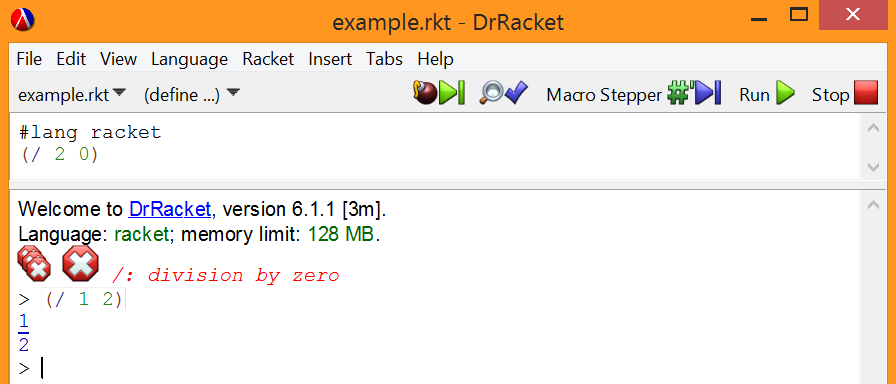
\includegraphics[keepaspectratio, width= 1.0 \textwidth]{drracketGUI.png}
		\end{itemize}
		
\end{frame}

\begin{frame}
	\frametitle{DrRacket interface}
			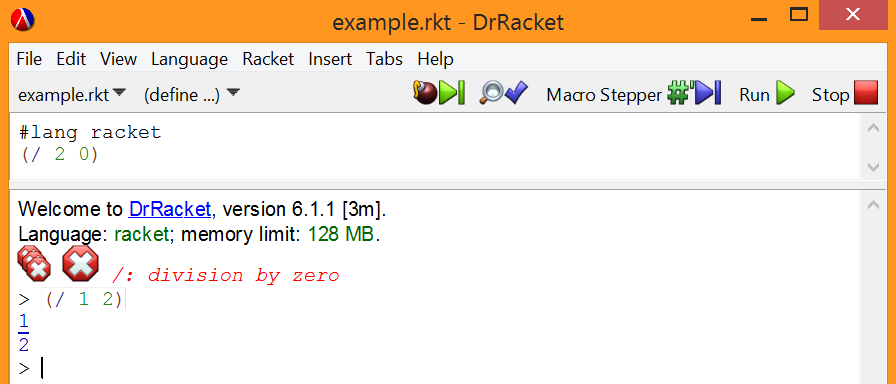
\includegraphics[keepaspectratio, width= 1.0 \textwidth]{drracketGUI.png}

\end{frame}

\begin{frame}
	\frametitle{Study of DrRacket error messages}
		\begin{itemize}
			\item Marceau et al. interested in finding which errors students struggled with
			\item Configured DrRacket to save a copy of each program a student tried to execute and the error messages received
			\item Programs taken from a once-per-week lab session
		\end{itemize} 

\end{frame}

\begin{frame}
	\frametitle{Table of results}
	\includegraphics[keepaspectratio, width=1.0 \textwidth]{MEE-data.pdf}

\end{frame}


\begin{frame}
	\frametitle{Results}
		\begin{itemize}
			\item Students struggle with certain errors relative to skill level
			\item Some errors were not indicator of underlying issue
			\begin{itemize}
			\item student struggled with these errors
			\item suggests issues in error message effectiveness
			\end{itemize}
		\end{itemize}

\end{frame}

\begin{frame}[fragile]
 \frametitle{Student code example}
 			\begin{verbatim}
(define (label-near? name bias word1 word2)
  (cond
      (and (cond [(string=? name word1) 
                    "Name Located"]
                 [(string=? bias word2)
                    "Bias Located"])
           (cond [(string=? name word2)
                    "Name Located"]
                 [(string=? bias word2) 
                    "Bias Located"])
     "Mark")
))

-> and: found a use of 'and' that does not follow 
an open parenthesis
			\end{verbatim}
\end{frame}

\subsection[Compiler Analysis]{Analysis of compiler errors}

\begin{frame}
	\frametitle{Overview of study}
		\begin{itemize}
			\item Compiler error messages often cryptic and difficult for many programmers
			\item Traver and his students found compiler errors messages difficult to understand
			\item Traver conducted study in Fall 2002 at Jaume I University to verify which errors intro students struggle with
				\begin{itemize}
				\item course used C++ programming language
				\end{itemize}
		\end{itemize}

\end{frame}

\begin{frame}[fragile]
	\frametitle{Intro to C++}
		\begin{itemize}
			\item Not designed to be taught in intro course
			\item Imperative language: uses memory manipulation and state-changing statements to build computation
			\item statically-typed
			\item Object-oriented programming (OOP): method of programming around class hierarchy and creating objects
			\item Syntax example:
			\begin{verbatim}
			int a = 2;
			a = a + 2;
			cout << a;
			-> 2
			\end{verbatim}
		\end{itemize}

\end{frame}

\begin{frame}
	\frametitle{Method of study}
		\begin{itemize}
			\item GNU g++ compiler was used
			\item Code gathered from students in lab sessions throughout semester
			\item Analyzed each message and wrote out the following for each message:
			\begin{itemize}
				\item why the error occurred
				\item possible alternate error message
				\item why the error is unhelpful
			\end{itemize}
		\end{itemize}

\end{frame}

\begin{frame}[fragile]
	\frametitle{Example of code analyzed}
Offending code:
\begin{verbatim}
SavingAccount::SavingAccount(){
    float SavingAccount::getInterestRate() {
   	  return rate;
}
\end{verbatim}

Error message:
\begin{verbatim}
In method 'SavingAccount::SavingAccount()':
declaration of 'float SavingAccount::getInterestRate()'
outside of class is not definition
\end{verbatim}

\end{frame}

\begin{frame}[fragile]
	\frametitle{Example continued}
Alternative error message:
\begin{verbatim}
A function declaration inside a function body is 
not possible. Did you forget '}' to close the 
body of the previous function definition?
\end{verbatim}

\end{frame}

\begin{frame}
	\frametitle{Results}
		\begin{itemize}
			\item Study makes a good case for compiler error usability
			\item Hopes that approaches be considered to improve messages
			\item Helped him understand which errors students students struggled with
		\end{itemize}

\end{frame}

\section[Methodologies]{Methodologies for improving error messages}

\subsection[DrRacket recommendations]{Recommendations for improving IDE error messages}

\begin{frame}
	\frametitle{Recommendations}
		\begin{itemize}
			\item Marceau et al. based their research on these 
			\item Wanted to maintain two design principles:
			\begin{itemize}
				\item error messages should not propose solutions
				\item error messages should not prompt toward incorrect edits
			\end{itemize}
		\end{itemize}

\end{frame}

\begin{frame}[fragile]
	\frametitle{recommendations continued}
		\begin{itemize}
			\item Simplify message vocabulary
				\begin{itemize}
					\item eg, student will understand \texttt{variable} more than \texttt{identifier}
					\item these should be for lower levels in DrRacket
				\end{itemize}
			\item Be explicit with constructor or function usage in highlighting
			\item Color coding references with its corresponding code
		\end{itemize}

\end{frame}

\begin{frame}
	\frametitle{Color coded error message}
	Red highlights definition, green highlights clause, blue highlights definition
	\center
		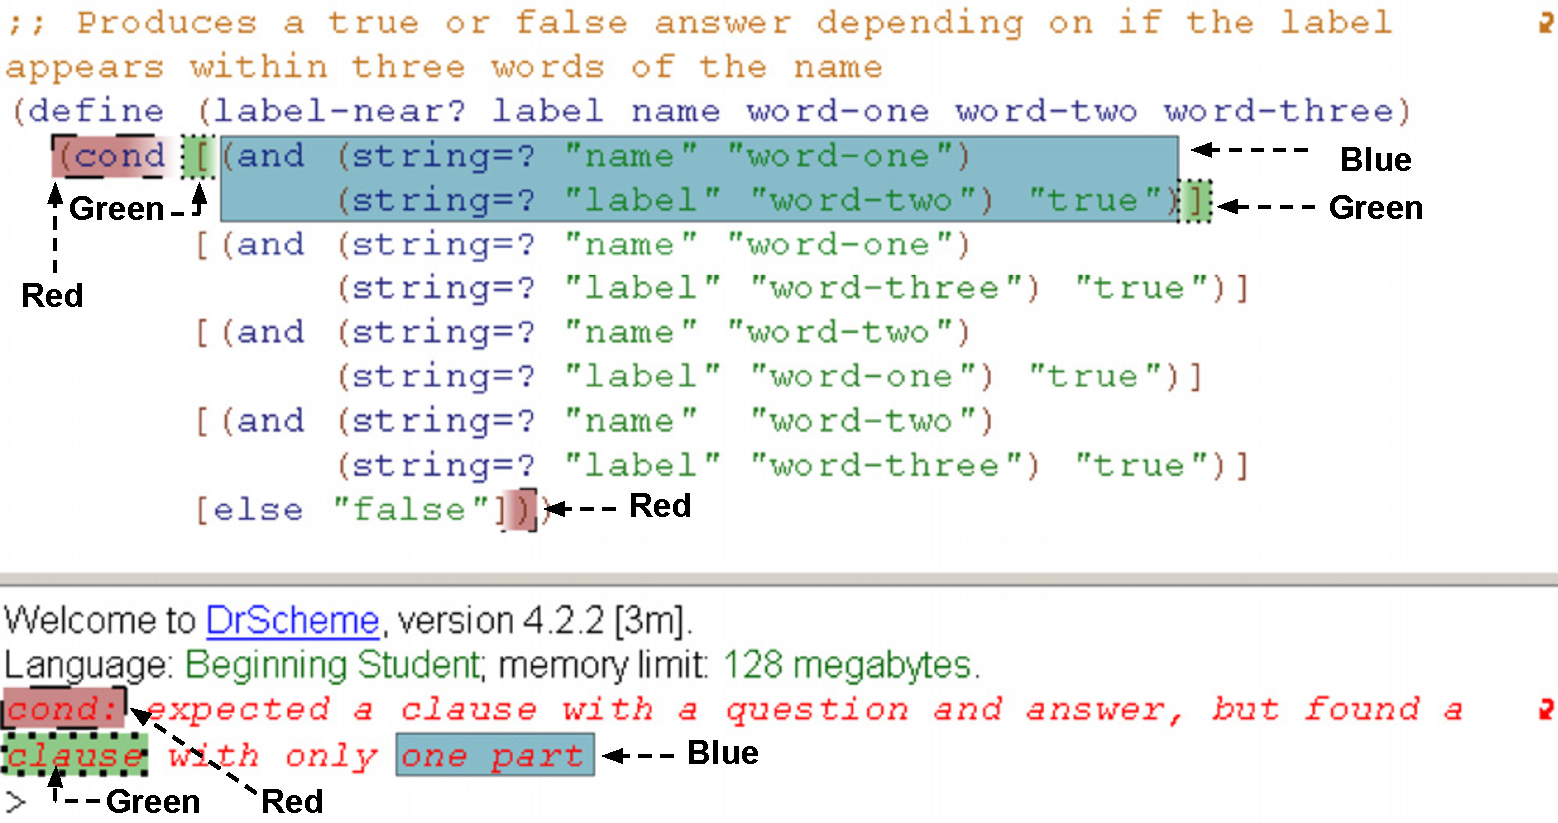
\includegraphics[keepaspectratio, width=0.8 \textwidth]{ColorCodedMessage.pdf}
\end{frame}

\begin{frame}
	\frametitle{Future work}
		\begin{itemize}
			\item Recommendations implemented in How to Design Programs (HtDP) libraries in DrRacket
			\item Further research needed to evaluate HtDP libraries
		\end{itemize}

\end{frame}

\subsection[Syntax error enhancement]{Analysis of syntax error enhancement}

\begin{frame}
	\frametitle{Intro to syntax errors}
		\begin{itemize}
			\item Introductory students most likely receive many syntax errors in first few weeks of learning language
			\item "Syntax errors are significant barrier to student success" - Denny et al.
			\item Denny et al. propose to improve syntax error messages in course
		\end{itemize}

\end{frame}

\begin{frame}
	\frametitle{Improving errors}
		\begin{itemize}
			\item Course used Java, language similar to C++
			\item Course also used CodeWrite, online IDE
			\item Pulled student submissions from CodeWrite
			\item Match commonly erroneous code, extracted line containing error, and inserted their enhanced error
		\end{itemize}

\end{frame}

\begin{frame}
	\frametitle{Enhanced syntax error example}
	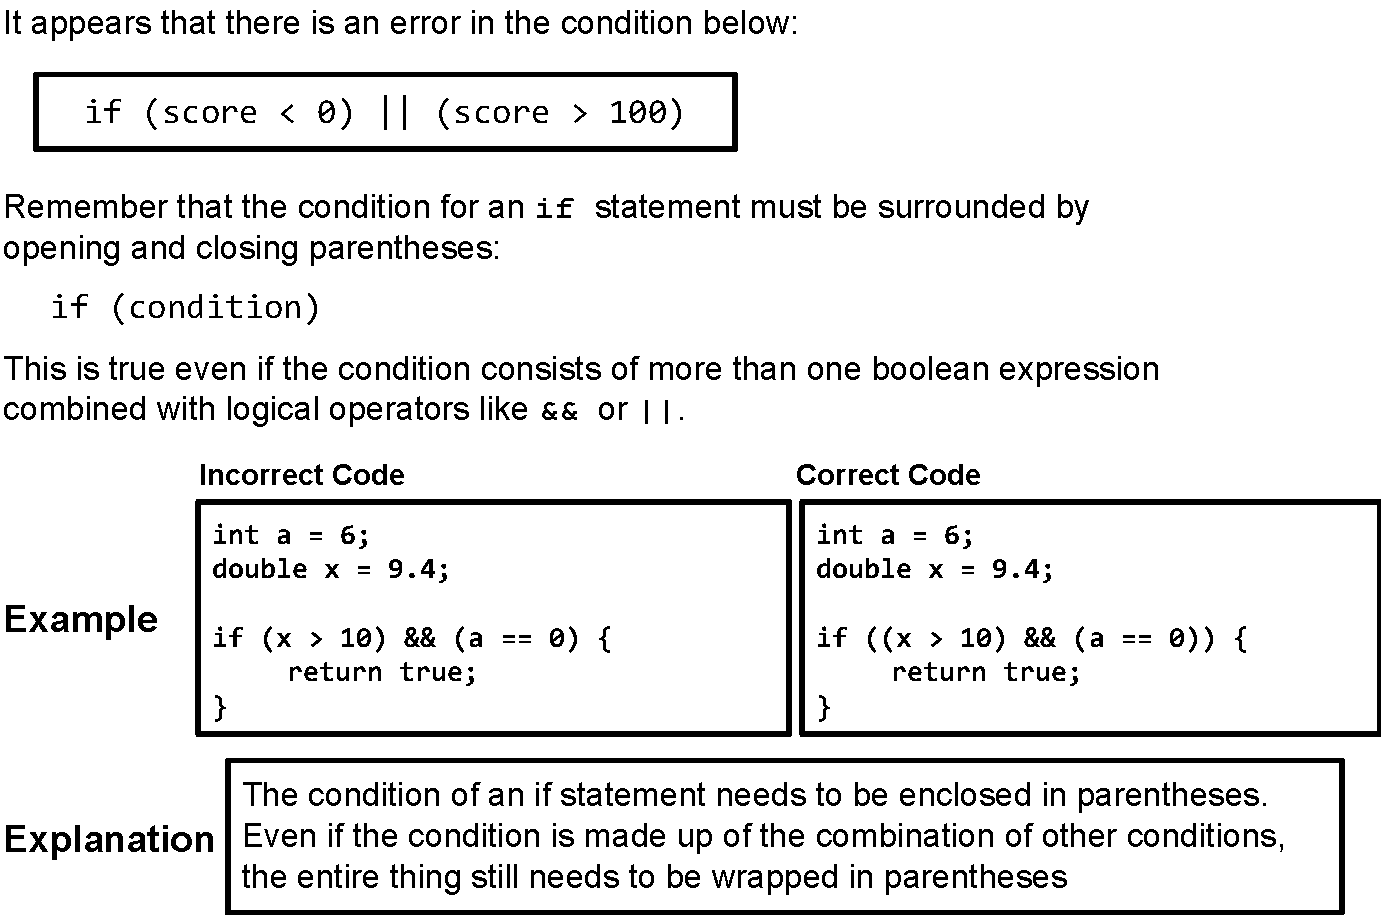
\includegraphics[keepaspectratio, width=0.8 \textwidth]{EnhancedSyntaxErrorSlide.pdf}
\end{frame}

\begin{frame}
	\frametitle{Testing the enhanced syntax messages}
		\begin{itemize}
			\item Students in control group (original error messages) and intervention group (enhanced error messages)
			\item Compared attempts of student submissions to see if it would reduce the number of non-compiling submissions overall
			\item Used t-tests to find results
			(still need to define t-test)
		\end{itemize}

\end{frame}

\begin{frame}
	\frametitle{Results of syntax enhancement}
		\begin{itemize}
			\item t-tests gave high p-values (p > 0.05)
				\begin{itemize}
				\item indication of no evidence of significant difference between the groups
				\end{itemize}
		\end{itemize}

\end{frame}

\begin{frame}
	\frametitle{Future work}
		\begin{itemize}
			\item Denny et al. believed several factors were cause for no significance
			\begin{itemize}
				\item for example, students may not have paid attention to additional information
			\end{itemize}
			\item Authors would like to apply additional research to improve their messages
		\end{itemize}

\end{frame}


\section[Conclusions]{Conclusions}

\begin{frame}
	\frametitle{Results}
		\begin{itemize}
			\item Some work needs to be done with DrRacket error messages to better report the actual errors
			\item Compiler error messages are an issue in terms of usability
			\item Research is being done in attempt to improve error messages
			\begin{itemize}
				\item Marceau et al. recommendations for error message design in IDEs
				\item Denny et al. syntax error message enhancement
			\end{itemize}
		\end{itemize}

\end{frame}

\begin{frame}
	\frametitle{Future work}
		\begin{itemize}
			\item HtDP libraries implemented Marceau et al. research
			\item Some work being done to attempt to improve compiler error messages
			\item Growing interest in computer science
			\begin{itemize}
				\item more user-friendly error messages are a necessity
			\end{itemize}
		\end{itemize}

\end{frame}

\begin{frame}
	\frametitle{Acknowledgments}
	I would like to thank the following people:
		\begin{itemize}
			\item My advisor, Elena Machkasova, for helping with my senior seminar and useful feedback on my paper and presentation
			\item Stephen Adams and Jim Hall for providing useful feedback on my paper
			\item Friends and family for attending
			\item Paul Schliep, as none of this would have been possible without him
		\end{itemize}

\end{frame}

\begin{frame}
	\frametitle{Thanks!}
	
	Thank you for your time and attention!
		
	\linespace
	\linespace
	
	Contact:  
	\begin{itemize}
		\item \texttt{schli202@morris.umn.edu}
		\item \url{github.com/Paul-Schliep}
	\end{itemize}
	
	\linespace
	\linespace
	
	\begin{center}
	{\huge Questions?}
	\end{center}
\end{frame}

\section*{References}

\begin{frame} 
	\frametitle{References} 
	
	\begin{thebibliography}{lskdjf}
	
	\bibitem{McPhee:2009:gecco}
Marceau, G., Fisler, K., and Krishnamurthi s.
\newblock Measuring the effectiveness of error messages designed for novice programmers.
\newblock In Proceedings of the 42nd ACM Technical Symposium on Computer Science Education, New York, NY, USA, 2011.
	
	\bibitem{citeulike:3452411}
	Traver, V.J.
\newblock On compiler error messages: What they say and what they mean.
\newblock In Advances in Human-Computer Interaction, 2010.
  
  	\end{thebibliography}
	
	\linespace
	\begin{center}
	See my senior seminar paper for additional references.
	\end{center}
\end{frame} 

\end{document}


